\documentclass[aspectratio=169, xcolor=dvipsnames]{beamer}

% --- Theme Setup ---
\usetheme{Madrid}
\usecolortheme{default}

% --- Packages ---
\usepackage{listings}
\usepackage{xcolor}
\usepackage{tikz}
\usetikzlibrary{shapes, arrows, positioning, fit}
\usepackage{booktabs}
\usepackage{tcolorbox}
\usepackage{amsmath}
\usepackage{hyperref}

% --- Code Highlighting Style ---
\definecolor{codegreen}{rgb}{0,0.6,0}
\definecolor{codegray}{rgb}{0.5,0.5,0.5}
\definecolor{codepurple}{rgb}{0.58,0,0.82}
\definecolor{backcolour}{rgb}{0.95,0.95,0.92}

\lstdefinestyle{mystyle}{
    backgroundcolor=\color{backcolour},   
    commentstyle=\color{codegreen},
    keywordstyle=\color{magenta},
    numberstyle=\tiny\color{codegray},
    stringstyle=\color{codepurple},
    basicstyle=\ttfamily\footnotesize,
    breakatwhitespace=false,         
    breaklines=true,                 
    captionpos=b,                    
    keepspaces=true,                 
    numbers=left,                    
    numbersep=5pt,                  
    showspaces=false,                
    showstringspaces=false,
    showtabs=false,                  
    tabsize=2,
    escapechar=|
}
\lstset{style=mystyle}

% --- Notes Setup ---
% Enable this to see notes in PDF if debug is needed, otherwise hide for video generation source
\setbeameroption{hide notes} 

% --- Section Popup ---
\AtBeginSection[]{
  \begin{frame}
  \vfill
  \centering
  \begin{beamercolorbox}[sep=8pt,center,shadow=true,rounded=true]{title}
    \usebeamerfont{title}\insertsectionhead\par%
  \end{beamercolorbox}
  \vfill
  \end{frame}
}

\title{Beamer Feature Showcase}
\subtitle{Comprehensive Reference for Automated slides}
\author{System Reference}
\date{\today}

\begin{document}

% ==========================================
% Title Slide
% ==========================================
\begin{frame}
    \titlepage
    \begin{center}
        \small This reference covers structure, content, visuals, and animation.
    \end{center}
    
    \note{
        [click] Dr. James: Welcome to the Comprehensive Beamer Feature Showcase.
        [click] Sarah: This document covers not just content, but structure, navigation, and visual styling logic.
    }
\end{frame}

% ==========================================
% Table of Contents
% ==========================================
\begin{frame}{Table of Contents}
    \tableofcontents
    \note{
        Dr. James: A table of contents is crucial for longer presentations. 
        [click] Sarah: Beamer generates this automatically from section commands.
    }
\end{frame}

% ==========================================
% SECTION 1: Structure & Layout
% ==========================================
\section{Structure \& Layout}

\begin{frame}{Incremental Reveals}
    To keep the video engaging, reveal content step-by-step using \texttt{<+->}.
    
    \begin{itemize}
        \item<1-> \textbf{Step 1}: Introduce the concept.
        \item<2-> \textbf{Step 2}: Expand on details.
        \item<3-> \textbf{Step 3}: Conclude the point.
    \end{itemize}
    
    \note{
        Dr. James: In our first section, Structure and Layout.
        [click] Dr. James: We start with incremental reveals to control pacing.
        [click] Sarah: Step two.
        [click] Sarah: And step three.
    }
\end{frame}

\begin{frame}[fragile]{Comparing Approaches (Columns)}
    Use columns to compare side-by-side.
    
    \begin{columns}
        \begin{column}{0.48\textwidth}
            \textbf{Approach A}
            \begin{lstlisting}[language=Python, basicstyle=\tiny\ttfamily]
def fib(n):
    if n <= 1: return n
    return fib(n-1) + fib(n-2)
            \end{lstlisting}
        \end{column}
        
        \begin{column}{0.48\textwidth}
            \textbf{Approach B}
            \begin{lstlisting}[language=Python, basicstyle=\tiny\ttfamily]
def fib(n):
    a, b = 0, 1
    for _ in range(n):
        a, b = b, a + b
    return a
            \end{lstlisting}
        \end{column}
    \end{columns}
    
    \note{
        Dr. James: Columns are essential for comparisons.
    }
\end{frame}

\begin{frame}{Beamer Blocks}
    Organize information using standard Beamer environment blocks.

    \begin{block}{Standard Block}
        This is a normal block for general information.
    \end{block}

    \begin{alertblock}{Alert Block}
        Use this for warnings or critical points.
    \end{alertblock}

    \begin{examples}
        This is an example block, useful for case studies.
    \end{examples}

    \note{
        Sarah: Beamer provides distinct block types.
        [click] Sarah: The standard block.
        [click] Dr. James: The alert block for emphasis.
        [click] Sarah: And the examples block.
    }
\end{frame}

% ==========================================
% SECTION 2: Rich Content
% ==========================================
\section{Rich Content}

\begin{frame}{Math \& Equations}
    Beamer handles complex math gracefully.
    
    \begin{itemize}
        \item Inline Math: $e^{i\pi} + 1 = 0$
        \item Block Equations with overlays:
    \end{itemize}
    
    \onslide<2->{
        \begin{align*}
            f(x) &= x^2 + 2x + 1 \\
            \onslide<3->{&= (x+1)^2}
        \end{align*}
    }

    \note{
        Dr. James: Moving to Rich Content. Math support is first class.
        [click] Sarah: We can reveal derivations step by step.
    }
\end{frame}

\begin{frame}[fragile]{Code Evolution}
    We can simulate "Magic Move" by showing code changes across overlays.
    
    \begin{onlyenv}<1>
        \begin{lstlisting}[language=Python, title={Initial State}]
def calculate_area(radius):
    pi = 3.14
    return pi * radius * radius
        \end{lstlisting}
    \end{onlyenv}
    
    \begin{onlyenv}<2>
        \begin{lstlisting}[language=Python, title={Refactored (Import Math)}]
import math

def calculate_area(radius):
    return math.pi * radius * radius
        \end{lstlisting}
    \end{onlyenv}

    \note{
        Sarah: Code evolution is crucial for technical talks.
        [click] Dr. James: We update the code in place using overlays.
    }
\end{frame}

\begin{frame}{Styled Components}
    Use \texttt{tcolorbox} to simulate modern UI components.
    
    \begin{tcolorbox}[colback=blue!5!white, colframe=blue!75!black, title=Info Card]
        This box mimics a standardized component style.
    \end{tcolorbox}
    
    \vspace{0.5cm}
    
    \begin{tcolorbox}[colback=yellow!10!white, colframe=orange!75!black, title=Alert Component]
        \textbf{Warning:} This is an important alert.
    \end{tcolorbox}

    \note{
        Dr. James: We can also create custom components like Info Cards.
        [click] Sarah: Or Alert Boxes.
    }
\end{frame}

% ==========================================
% SECTION 3: Visuals & Navigation
% ==========================================
\section{Visuals \& Navigation}

\begin{frame}{Digrams (TikZ)}
    \centering
    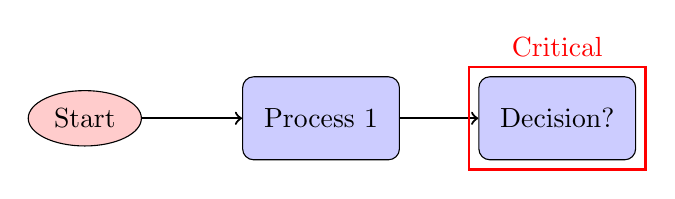
\begin{tikzpicture}[node distance=2cm, auto]
        \tikzstyle{block} = [rectangle, draw, fill=blue!20, text width=5em, text centered, rounded corners, minimum height=3em]
        \tikzstyle{cloud} = [draw, ellipse, fill=red!20, minimum height=2em]
        
        \node [cloud] (start) {Start};
        \node [block, right of=start, node distance=3cm] (proc1) {Process 1};
        \node [block, right of=proc1, node distance=3cm] (decision) {Decision?};
        
        \path [draw, ->, thick] (start) -- (proc1);
        \path [draw, ->, thick] (proc1) -- (decision);
        
        \onslide<2->{
             \node[draw, red, thick, fit=(decision), label=above:\textcolor{red}{Critical}] {};
        }
    \end{tikzpicture}

    \note{
        Dr. James: Vector diagrams are rendered natively.
        [click] Sarah: And can be highlighted dynamically.
    }
\end{frame}

\begin{frame}{Navigation Buttons}
    Beamer supports interactive buttons.
    
    \centering
    \hyperlink{transitions}{\beamerbutton{Jump to Transitions}}
    \vspace{1cm}
    \hyperlink{transitions}{\beamergotobutton{Go to Transitions}}
    
    \note{
        Dr. James: Interactive elements like buttons allow for non-linear presentations.
        [click] Sarah: Typically less used in linear video, but valuable for reference.
    }
\end{frame}

% ==========================================
% SECTION 4: Animation
% ==========================================
\section{Animation}

\begin{frame}[label=transitions]{Transitions}
    \transdissolve<1>
    This slide used a \texttt{dissolve} transition to appear.
    
    \vspace{1em}
    Other standard transitions:
    \begin{itemize}
        \item \texttt{transblindshorizontal}
        \item \texttt{transboxin}
        \item \texttt{transglitter}
    \end{itemize}

    \note{
        Dr. James: Finally, animation.
        Sarah: Use transitions sparingly, but they add polish.
    }
\end{frame}

\end{document}
